\section{Outlook}\label{sec:outlook}
% features of the application

% What did I find?
When investigating both semantic and visual embedding methods, differences between the models became evident.
Overall, the textual embedding methods produced more meaningful responses than the visual embedding methods.
However, this is not surprising since the textual embedding methods prioritize documents containing equal or semantically similar terms and thus,
return documents of similar content or originating from the same company as the query document.
Visual embedding methods, on the other hand, return visually similar documents.

It is complicated to compare the responses of semantic and visual embedding methods since they operate on fundamentally different data.
A more thorough evaluation could include a survey.
A selection of the results of this work is incorporated into the first approach to constructing a survey.
13 people with different academic backgrounds have partaken in the survey.
A question and result from the survey are displayed in \autoref{fig:survey}.
However, constructing a survey is complicated since semantic similarities should be evaluated on a textual level, i.e.\ content, 
which is difficult for non-experts and not natural since humans are prone to assess similarities by visual inspection.
Moreover, identification of the target audience is difficult since the target audience of the tool could be expanded to be more general than the tax office.

\begin{figure}%
    \centering
    \subfloat[\centering A question of the survey.]{{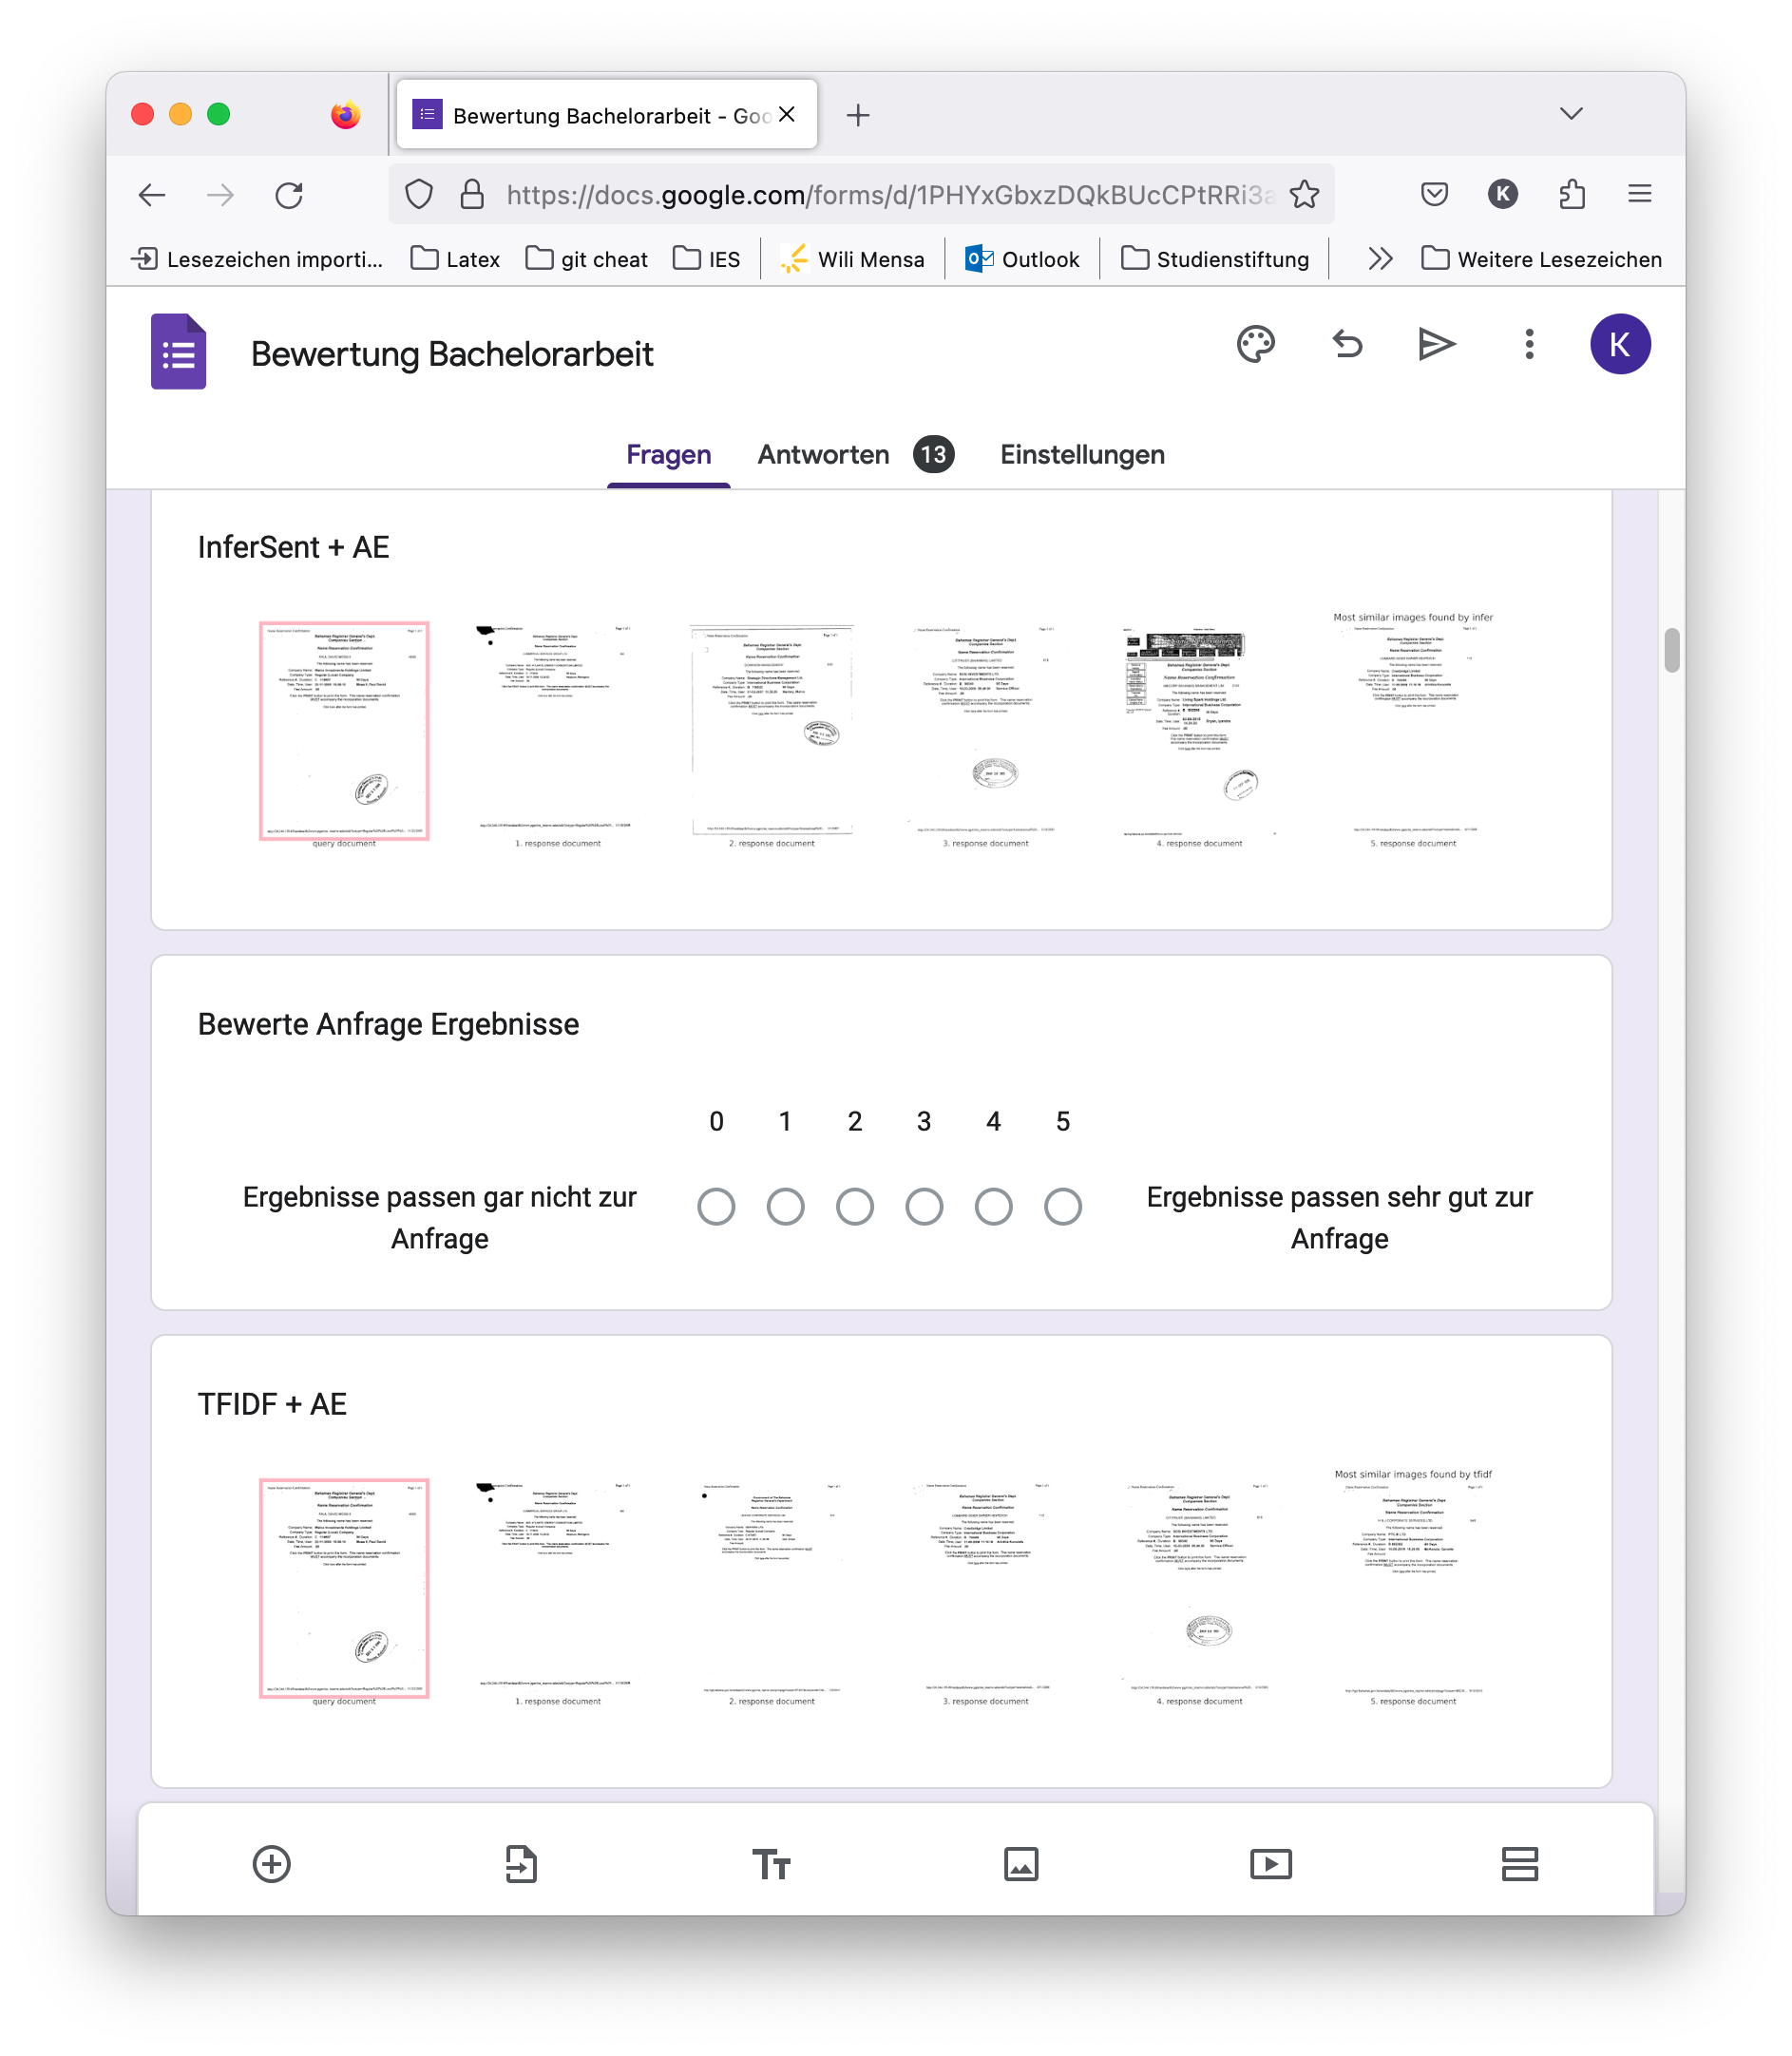
\includegraphics[width=5cm]{images/Umfrage/Umfrage_ex.png} }}%
    \qquad
    \subfloat[\centering Selection of results of survey.]{{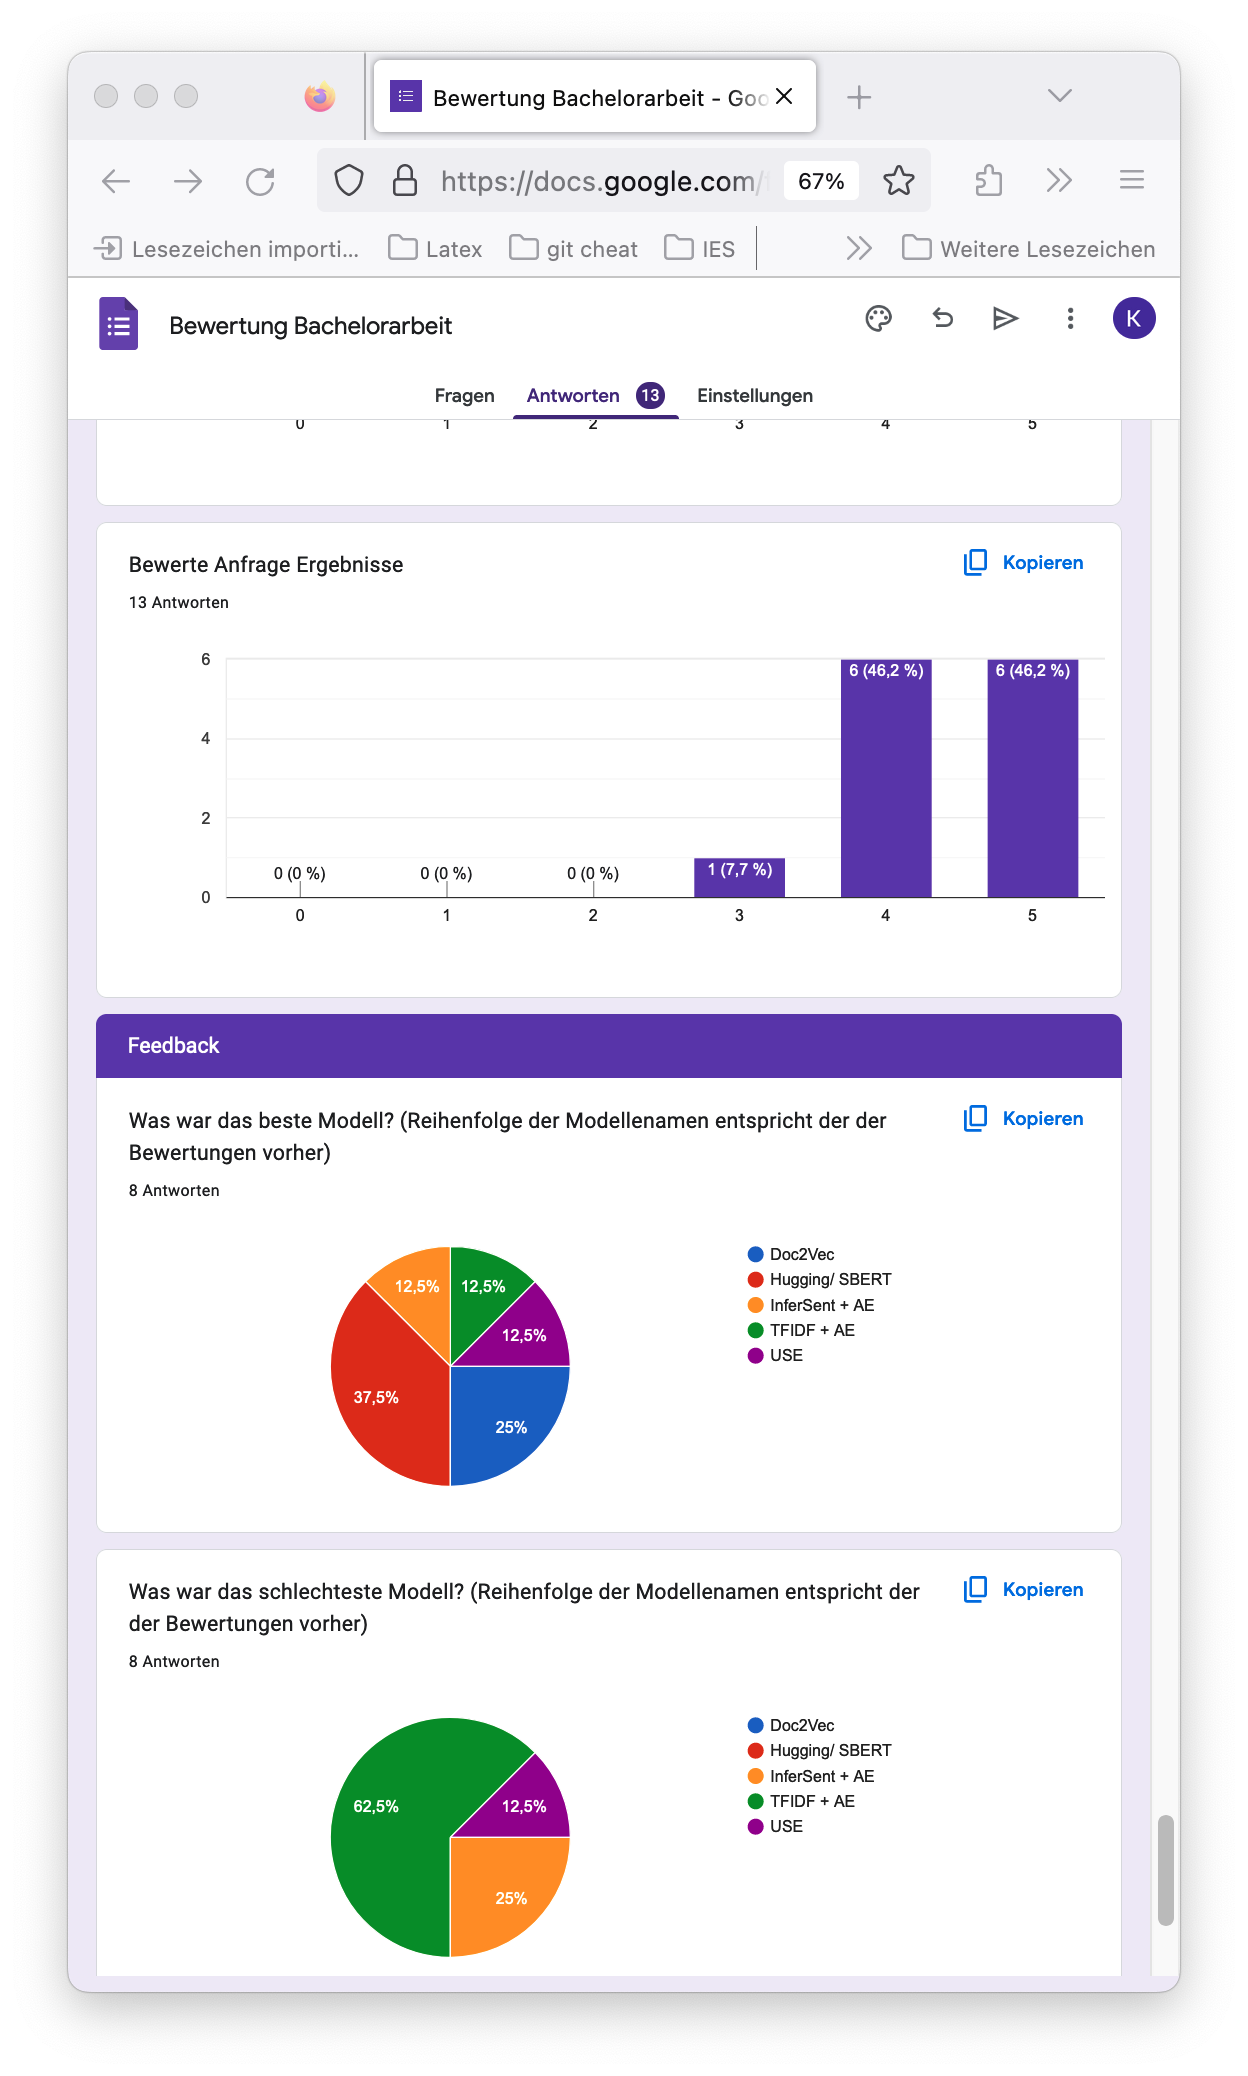
\includegraphics[width=5cm]{images/Umfrage/Umfrage_erg.png} }}%
    \caption[Survey approach]{A first survey approach from \cite{BA-survey}.}%
    \label{fig:survey}%
\end{figure}

% Problems/ critic
% Embedding methods
% hyperparameter tuning
Similar to \citeauthor{glove2014}'s work, in this thesis, for many models used, any unspecified parameters are set to their default values, 
assuming that they are close to optimal
acknowledging that this simplification should be revised in a more thorough analysis.

% TFIDF
The \ac{tfidf} approach performs rather poorly on unusual query documents.
There are multiple factors that could have contributed to this result.
Firstly, the vocabulary is drastically reduced to satisfy the database's constraints for dense vector dimensionality.
Thus, \ac{tfidf} may either be unsuitable for the task of finding similar documents when the vocabulary size is restricted or 
further research is required to find more suitable means to compress the embedding before inserting it into the database.
Secondly, the evaluation of the different preprocessors of \ac{tfidf} is carried out on small datasets of 195 and 2048 documents.
This dataset may not be representative of the whole corpus.

% GloVe (InferSent)
In this work, the precomputed \ac{glove} embeddings are replaced by a custom \ac{w2v} model.
However, \citeauthor{glove2014} state that \acs{glove} outperforms \ac{w2v} on the same corpus, 
vocabulary and window size in terms of quality \cite{glove2014}.
Hence, the quality of \infersent{} might have deteriorated due to the replacement of \ac{glove} by \ac{w2v}.

% Visual embedding methods
% Eigendocs
When preprocessing the document images for \eigendocs{}, the images are placed on a white canvas assuming 
its dimensions are bigger or equal to all other documents in the corpus.
Since this assumption was not true, the images selected to find the dimensionalities of the canvas are not representative.

% compression: PCA
The parameter selection for \ac{pca} is not representative of the whole dataset, 
due to the fact that the dataset used for the evaluation error was not drawn randomly from the data corpus and is too small.
Moreover, the resulting plot is not optimal for conducting the "elbow method", since no significant change is evident in the slope.


% AE config: Problem & future work
Different \ac{ae} architectures are experimentally evaluated on a selection of 195 documents.
However, since the dataset is too small and not drawn randomly from the whole data corpus the results are not representative.
Thus, future work should include a more thorough evaluation of different \ac{ae} architectures on a bigger document corpus.
% tfidf + AE only used on server

% comparison on training data
The comparison of the different embedding methods in terms of query response similarity was carried out on the data which was stored in the database.
For future work, the comparison should be carried out on a separate data set to evaluate the performance of the models on unseen data.

% eval weights of response documents
The evaluation of the similarity between query results of different models so far 
has not considered the individual weights for respective query responses
because it was difficult to find means 
to interpret and visualize semantic meaningful weight relationships.
Thus, future work could include the weights of the query responses in the evaluation.

% similarity of query documents
Moreover, the similarity of the query documents is not considered in the evaluation.
To further improve the evaluation, the number of occurrences of query documents in the response documents of other queries could be examined.
Another approach to evaluation could be to assess the quality of the images which were returned by multiple models.
Possibly, one could create a hypothesis about whether better responses correlate with the number of models that returned them.

% elastic stack: Kibana
The elastic stack offers a wide range of tools, for instance, Kibana that can be used to manage models and 
to create ingest pipelines to embed new documents.
If models are managed by Kibana, the models no longer have to be managed by the user and thus, 
the system would most likely be more user-friendly and less prone to errors.

% server database
Another issue is the fact that the database contains neither all embeddings nor all documents.
The Bahamas leak contains 38 \ac{gb} of data.
Even though multiprocessing using Pool is used to split the workload across up to 100 processes, 
the embedding process is not finished after several days.
Hence, more advanced coding techniques have to be applied to speed up the embedding process.

% Future: continue developing this application with the tax office
The domain of financial fraud and tax evasion is very interesting.
Thus, future work could include the development of a working system for the tax office.
The techniques explored in this work could be used to find similar documents to a query document and thus,
facilitate initial exploration of a large data corpus.
However, the tool developed in this work is not yet ready to be used in tax offices.
The different embedding models to choose from are useful for research purposes but not in a productive environment.